\documentclass[14pt]{extbook}
\usepackage{multicol, enumerate, enumitem, hyperref, color, soul, setspace, parskip, fancyhdr} %General Packages
\usepackage{amssymb, amsthm, amsmath, latexsym, units, mathtools} %Math Packages
\everymath{\displaystyle} %All math in Display Style
% Packages with additional options
\usepackage[headsep=0.5cm,headheight=12pt, left=1 in,right= 1 in,top= 1 in,bottom= 1 in]{geometry}
\usepackage[usenames,dvipsnames]{xcolor}
\usepackage{dashrule}  % Package to use the command below to create lines between items
\newcommand{\litem}[1]{\item#1\hspace*{-1cm}\rule{\textwidth}{0.4pt}}
\pagestyle{fancy}
\lhead{Progress Quiz 1}
\chead{}
\rhead{Version A}
\lfoot{3629-3146}
\cfoot{}
\rfoot{Summer C 2021}
\begin{document}

\begin{enumerate}
\litem{
Write the equation of the line in the graph below in Standard Form $Ax+By=C$. Then, choose the intervals that contain $A, B, \text{ and } C$.
\begin{center}
    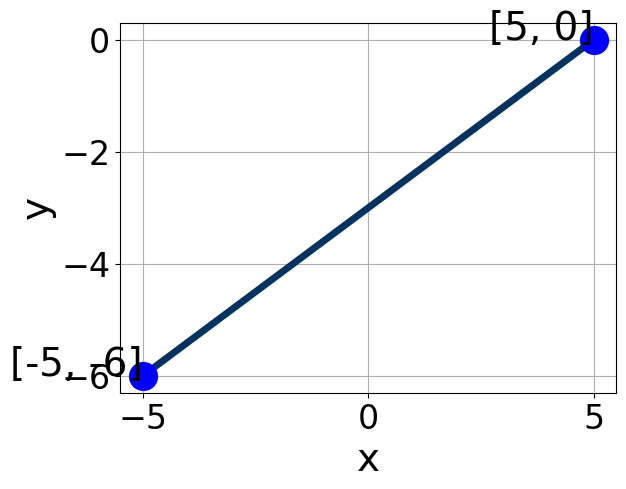
\includegraphics[width=0.5\textwidth]{../Figures/linearGraphToStandardA.png}
\end{center}
\begin{enumerate}[label=\Alph*.]
\item \( A \in [-0.1, 4.5], \hspace{3mm} B \in [4.6, 8], \text{ and } \hspace{3mm} C \in [-16, -12] \)
\item \( A \in [-1.8, -0.5], \hspace{3mm} B \in [-1.9, 0.2], \text{ and } \hspace{3mm} C \in [3, 8] \)
\item \( A \in [-1.8, -0.5], \hspace{3mm} B \in [0.3, 2.3], \text{ and } \hspace{3mm} C \in [-8, 2] \)
\item \( A \in [-5.1, -2.3], \hspace{3mm} B \in [4.6, 8], \text{ and } \hspace{3mm} C \in [-16, -12] \)
\item \( A \in [-0.1, 4.5], \hspace{3mm} B \in [-5.7, -4.3], \text{ and } \hspace{3mm} C \in [10, 21] \)

\end{enumerate} }
\litem{
Find the equation of the line described below. Write the linear equation in the form $ y=mx+b $ and choose the intervals that contain $m$ and $b$.\[ \text{Perpendicular to } 7 x - 8 y = 5 \text{ and passing through the point } (10, 9). \]\begin{enumerate}[label=\Alph*.]
\item \( m \in [-1.6, -0.99] \hspace*{3mm} b \in [19.4, 20.9] \)
\item \( m \in [-1.6, -0.99] \hspace*{3mm} b \in [-21.4, -18.8] \)
\item \( m \in [-1.6, -0.99] \hspace*{3mm} b \in [-1.3, 0.8] \)
\item \( m \in [-1, -0.6] \hspace*{3mm} b \in [19.4, 20.9] \)
\item \( m \in [0.64, 1.8] \hspace*{3mm} b \in [-3.4, -1.8] \)

\end{enumerate} }
\litem{
Solve the linear equation below. Then, choose the interval that contains the solution.\[ \frac{-6x -5}{7} - \frac{-7x + 5}{2} = \frac{4x -5}{4} \]\begin{enumerate}[label=\Alph*.]
\item \( x \in [-1.2, -0.5] \)
\item \( x \in [2.8, 3.7] \)
\item \( x \in [-3, -1.3] \)
\item \( x \in [0.1, 2.9] \)
\item \( \text{There are no real solutions.} \)

\end{enumerate} }
\litem{
Write the equation of the line in the graph below in Standard Form $Ax+By=C$. Then, choose the intervals that contain $A, B, \text{ and } C$.
\begin{center}
    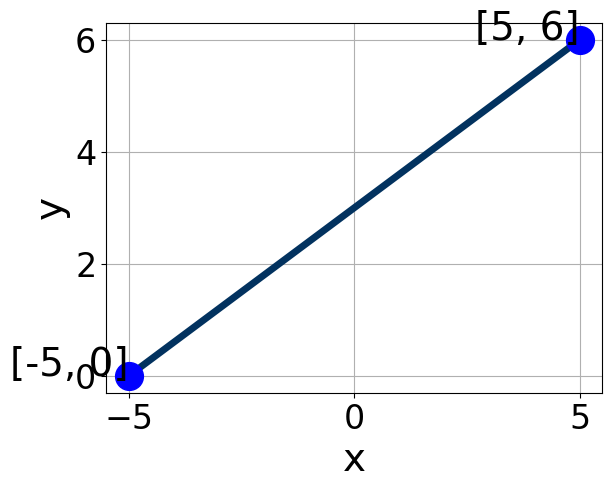
\includegraphics[width=0.5\textwidth]{../Figures/linearGraphToStandardCopyA.png}
\end{center}
\begin{enumerate}[label=\Alph*.]
\item \( A \in [-1.6, 2.4], \hspace{3mm} B \in [-2.4, -0.9], \text{ and } \hspace{3mm} C \in [-3, 2] \)
\item \( A \in [-1.6, 2.4], \hspace{3mm} B \in [0.2, 1.3], \text{ and } \hspace{3mm} C \in [-1, 4] \)
\item \( A \in [-4, -1], \hspace{3mm} B \in [4.1, 7.1], \text{ and } \hspace{3mm} C \in [15, 20] \)
\item \( A \in [2, 5], \hspace{3mm} B \in [4.1, 7.1], \text{ and } \hspace{3mm} C \in [15, 20] \)
\item \( A \in [2, 5], \hspace{3mm} B \in [-6.2, -4.8], \text{ and } \hspace{3mm} C \in [-17, -14] \)

\end{enumerate} }
\litem{
Find the equation of the line described below. Write the linear equation in the form $ y=mx+b $ and choose the intervals that contain $m$ and $b$.\[ \text{Parallel to } 5 x + 9 y = 15 \text{ and passing through the point } (-4, 8). \]\begin{enumerate}[label=\Alph*.]
\item \( m \in [-1.2, -0.25] \hspace*{3mm} b \in [11.1, 12.1] \)
\item \( m \in [-1.2, -0.25] \hspace*{3mm} b \in [4.7, 7.7] \)
\item \( m \in [-1.2, -0.25] \hspace*{3mm} b \in [-6.8, -4.5] \)
\item \( m \in [-2.76, -1.62] \hspace*{3mm} b \in [4.7, 7.7] \)
\item \( m \in [0.28, 1.49] \hspace*{3mm} b \in [10, 10.3] \)

\end{enumerate} }
\litem{
Solve the linear equation below. Then, choose the interval that contains the solution.\[ \frac{-7x -6}{6} - \frac{-7x -6}{5} = \frac{-3x -7}{7} \]\begin{enumerate}[label=\Alph*.]
\item \( x \in [-1.16, 0.31] \)
\item \( x \in [-11.22, -9.83] \)
\item \( x \in [0.78, 2.83] \)
\item \( x \in [-2.53, -1.78] \)
\item \( \text{There are no real solutions.} \)

\end{enumerate} }
\litem{
First, find the equation of the line containing the two points below. Then, write the equation in the form $ y=mx+b $ and choose the intervals that contain $m$ and $b$.\[ (-3, 6) \text{ and } (7, -11) \]\begin{enumerate}[label=\Alph*.]
\item \( m \in [-3.5, -0.8] \hspace*{3mm} b \in [-0.4, 4.1] \)
\item \( m \in [-3.5, -0.8] \hspace*{3mm} b \in [-19.6, -14.5] \)
\item \( m \in [1.6, 3] \hspace*{3mm} b \in [-25.8, -21.7] \)
\item \( m \in [-3.5, -0.8] \hspace*{3mm} b \in [-3.2, -0.1] \)
\item \( m \in [-3.5, -0.8] \hspace*{3mm} b \in [6.1, 10.3] \)

\end{enumerate} }
\litem{
Solve the equation below. Then, choose the interval that contains the solution.\[ -12(5x -2) = -9(15x + 7) \]\begin{enumerate}[label=\Alph*.]
\item \( x \in [-1.35, -1.05] \)
\item \( x \in [0.34, 0.63] \)
\item \( x \in [-0.53, -0.24] \)
\item \( x \in [-0.31, -0.12] \)
\item \( \text{There are no real solutions.} \)

\end{enumerate} }
\litem{
First, find the equation of the line containing the two points below. Then, write the equation in the form $ y=mx+b $ and choose the intervals that contain $m$ and $b$.\[ (-8, 5) \text{ and } (8, 4) \]\begin{enumerate}[label=\Alph*.]
\item \( m \in [-0.4, -0.02] \hspace*{3mm} b \in [12.97, 13.53] \)
\item \( m \in [0.04, 0.09] \hspace*{3mm} b \in [3.45, 4.08] \)
\item \( m \in [-0.4, -0.02] \hspace*{3mm} b \in [3.96, 4.57] \)
\item \( m \in [-0.4, -0.02] \hspace*{3mm} b \in [-4.05, -3.8] \)
\item \( m \in [-0.4, -0.02] \hspace*{3mm} b \in [-4.61, -4.44] \)

\end{enumerate} }
\litem{
Solve the equation below. Then, choose the interval that contains the solution.\[ -14(13x + 18) = -17(-4x -9) \]\begin{enumerate}[label=\Alph*.]
\item \( x \in [-0.79, 0.13] \)
\item \( x \in [-1.73, -1.55] \)
\item \( x \in [-1.15, -0.65] \)
\item \( x \in [0.34, 0.59] \)
\item \( \text{There are no real solutions.} \)

\end{enumerate} }
\end{enumerate}

\end{document}